\documentclass[12pt,onecolumn]{article}


\usepackage{float}
\usepackage{mathtools}
\usepackage[russian]{babel}
\everymath{\displaystyle}

\usepackage[usenames]{color}
\usepackage{colortbl}

\usepackage{geometry}
\geometry{
  a4paper,
  top=25mm, 
  right=30mm, 
  bottom=25mm, 
  left=30mm
}

\begin{document}

\begin{center}
    Санкт-Петербургский Национальный Исследовательский\\ 
    Университет ИТМО\\
    Факультет Программной Инженерии и Компьютерной Техники\\
    % \includegraphics{itm.jpg}
\end{center}
\vspace{1cm}


\begin{center}
    \large \textbf{Вариант №311809}\\
    \textbf{Лабораторная работа №1}\\
    по дисциплине\\
    \textbf{\textcolor{red}{\textit{'Программирование'}}}
\end{center}

\vspace{2cm}

\begin{flushright}
  Выполнил Студент  группы P3118\\
  \textbf{Михеев Илья}\\
  Преподаватель: \\
  \textbf{Письмак Алексей Евгеьевич}\\
\end{flushright}

\vspace{6cm}
\begin{center}
    г. Санкт-Петербург\\
    2021г.
\end{center}

\newpage
\section{Текст задания}
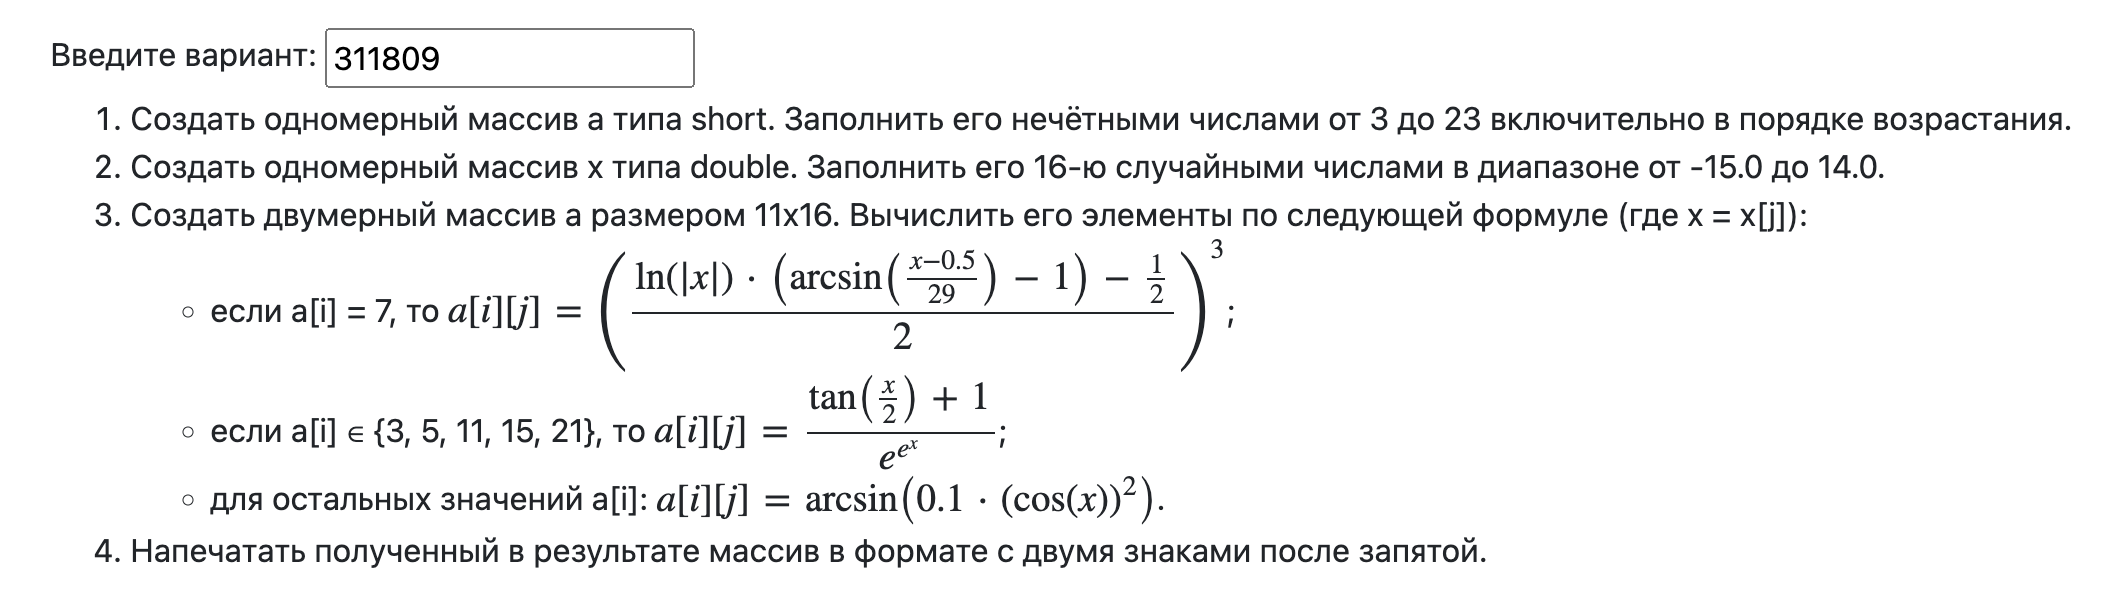
\includegraphics{task.png}

\section{Исходный код программы}
https://github.com/Ne0Ment/ITMO-proga/lab1/

\section{Результат выполнения}
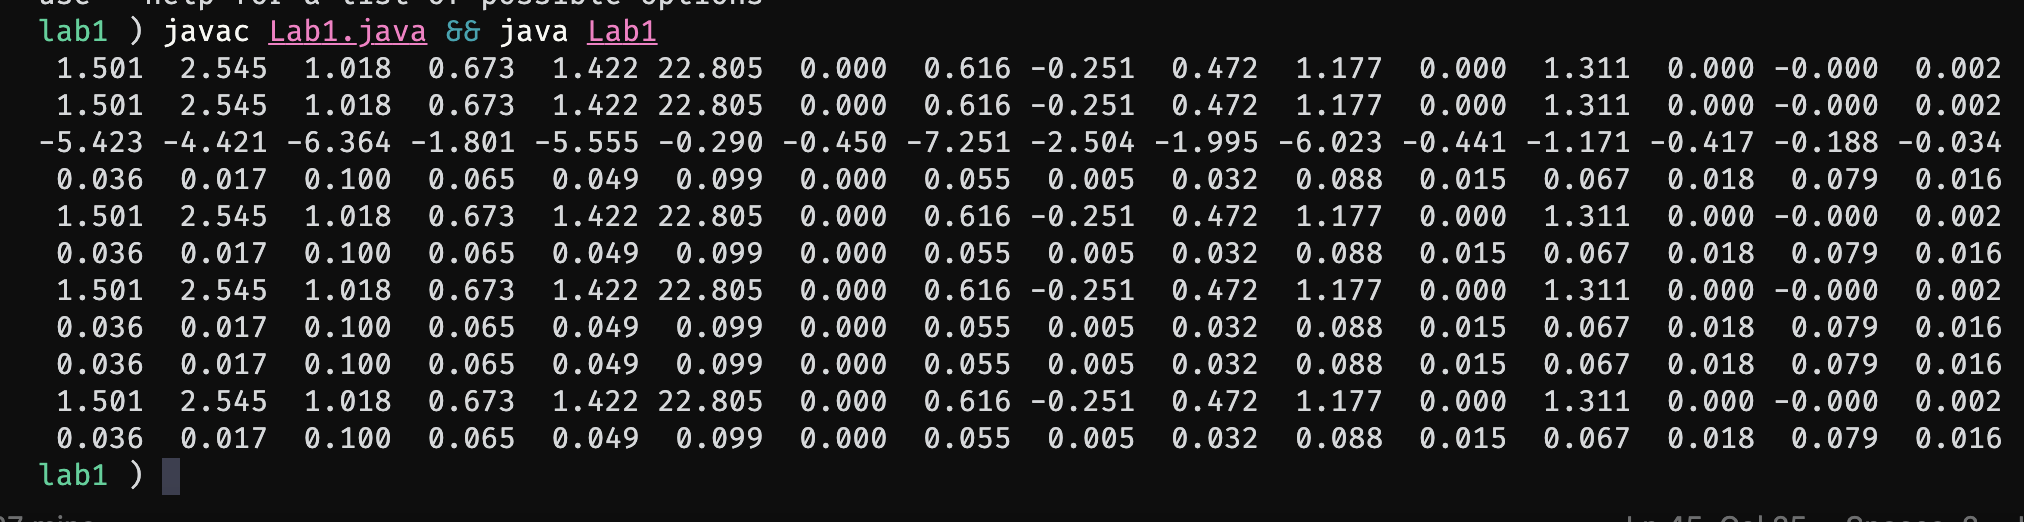
\includegraphics{result.png}

\section{Вывод}
Во время выполнения лабораторной работы я научился инициализировать переменные, использовать инструкции ветвления, циклы и функционал библиотеки java.lang.Math, а также инструментам JDK и JRE.

\end{document}